\documentclass{beamer}

\usepackage{beamerthemesplit}
\usetheme{Singapore} %Copenhagen}
%\usecolortheme{whale}

%\usepackage[T2A]{fontenc}
%\usepackage[utf8]{inputenc}
%\usepackage[russian]{babel}

\input{../../include/preamble.inc} 
\input{../../include/definitions.inc} 
\input{../../include/author.inc} 

\usepackage{enumitem}


%
%
%
%\newcommand{\argxi}{(\xi^1,\xi^2,\xi^3)}
%\newcommand{\argx}{(x^1,x^2,x^3)}
%
%\newcommand{\argxiv}{(\vec{\xi})}
%\newcommand{\argxv}{(\vec{x})}
%
%
%\newcommand{\argxbarn}{(\bar{x}^1,\bar{x}^2,\ldots, \bar{x}^n)}
%\newcommand{\argxn}{(x^1, x^2,\ldots, x^n)}
%
%\newcommand{\argtxi}{(t, \xi^1,\xi^2,\xi^3)}
%\newcommand{\argtoxi}{(t_0, \xi^1,\xi^2,\xi^3)}
%
%\newcommand{\argtxiv}{(t, \vec{\xi})}
%\newcommand{\argtoxiv}{(t_0, \vec{\xi})}
%
%
%\newcommand{\argtx}{(t, x^1,x^2,x^3)}
%\newcommand{\argtox}{(t_0, x^1,x^2,x^3)}
%
%\newcommand{\argtxv}{(t, \vec{x})}
%\newcommand{\argtoxv}{(t_0, \vec{x})}
%
%
%\newcommand{\pd}[2]{\frac{\partial #1}{\partial #2}}
%\newcommand{\pdk}[2]{\frac{\partial^2 #1}{\partial #2^2}}


\title[]{Классические модели механики жидкости и газа в рамках континуального подхода}

\author[]{ {\em Верещагин Антон Сергеевич}
\\
канд. физ.-мат. наук, старший преподаватель\\
\bigskip
Кафедра аэрофизики и газовой динамики ФФ НГУ}

\usebackgroundtemplate{
\includegraphics[width=\paperwidth]{../img/background.png}}

\begin{document}
	
\frame[plain]{\titlepage}


\frame[plain]{
	\frametitle{Аннотация}
	\parbox{\textwidth}{
		Жидкость, газ, твёрдое тело основные отличия. Идеальные, не идеальные и линейные и нелинейные среды. Модели идеальной несжимаемой жидкости, идеального политропного нетеплопроводного газа, вязкой несжимаемой жидкости, вязкого сжимаемого теплопроводного газа.
	}
}

\frame{
	\frametitle{ Жидкость, газ, твёрдое тело }
	
	\begin{exampleblock}{}
		\parbox{\textwidth}{
			\centering
			\Huge
			В чём отличие?
		}
	\end{exampleblock}
	
}


\frame{
	\frametitle{ Жидкость, газ, твёрдое тело }
	
	\begin{tabular}{p{2.5cm}|p{2cm}|p{2cm}|p{2cm}}
		\bf Свойство &  \bf  Газ & \bf Жидкость&  \bf Твёрдое тело \\
		\hline
		
		\em Сжимаемость & сильная & очень слабая &  практически отсутствует \\
		\hline
		\em Анизотропия &  нет & нет & бывает \\
		\hline
		\em Внутренние напряжения & функции градиента скорости (при наличие вязкости) & функции градиента скорости (при наличии вязкости) & функции градиента перемещений \\
		
		
	\end{tabular}
	
}

\frame{
	\frametitle{ Идеальные и не идеальные среды }
	
	\begin{columns}
		\begin{column}{0.7\textwidth}
			\begin{exampleblock}{Идеальная среда}
				\parbox{\textwidth}{
					Идеальная среда -- это такая среда, в которой отсутствует тангенциальная составляющая вектора напряжения $\vec{\sigma}_{n\tau}$ на любой площадке с нормалью $\vec{n}$, отвечающая за трение между слоями сплошной среды. При этом 
					\[
					\vec{\sigma}_{n}\argxv = -p\argxv\vec{n}.
					\] 
					Функция $p\argxv$ определяет давление в точке $\vec{x}$.
				}
			\end{exampleblock}
		\end{column}
		\begin{column}{0.3\textwidth}
			\centering
			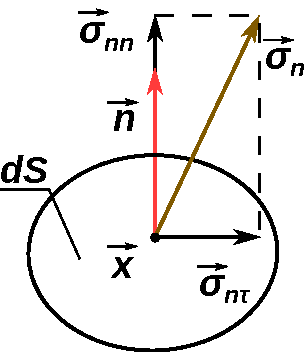
\includegraphics[width=\textwidth]{../img/sigma_decomposition.pdf}
			\[
			\vec{\sigma}_n = \vec{\sigma}_{nn}+\vec{\sigma}_{n\tau}
			\]
		\end{column}
	\end{columns}
}

\frame{
	\frametitle{ Линейные и нелинейные среды }
	
	\begin{exampleblock}{Линейность среды}
		\parbox{\textwidth}{
			Сплошная среды называется \alert{линейной}, если имеет место линейная зависимость между напряжениями возникающими в ней и изменениями деформаций или изменениями скоростей деформаций.
			
			\medskip
			Для {\em твёрдых тел} имеет место обобщённый закон Гука:
			\[
			\sigma_{ij} = C_{ijkm}\varepsilon_{km},\quad
			\varepsilon_{km} = \frac{1}{2}\left(\pd{u_k}{x_m} + \pd{u_m}{x_k} \right).
			\]
			
			\medskip
			Для {\em жидкостей или газов}:
			\[
			\sigma_{ij} = -p\delta_{ij} +  D_{ijkm}e_{km},\quad
			e_{km} = \frac{1}{2}\left(\pd{v_k}{x_m} + \pd{v_m}{x_k} \right).
			\]
			 Такие жидкости и газы называются \alert{ньютоновскими}. 
			
			
		}
		
	\end{exampleblock}
	
}

\frame{
	\frametitle{ Идеальная несжимаемая жидкость }
	
	\begin{exampleblock}{Основные допущения}
		\parbox{\textwidth}{
		\begin{itemize}[partopsep=1pt,label=\textbullet]
		\item Постоянная плотность среды
		\[
			\rho=const
		\]
			
		\item Напряжение на площадке c произвольной нормалью одинаково и направлено вдоль неё
		\[
		\sigma_{ij} = -p \delta_{ij}.
		\]
		
		В этом случае для любого вектора $\vec{n}$ единичной длины
		\[
		\vec{\sigma}_n = \vec{n} \cdot \sigma = -p\vec{n}.
		\]
		
			
		\end{itemize}	
			
		}
	\end{exampleblock}
	
}




\frame{
	\frametitle{ Идеальная несжимаемая жидкость }
	
	\begin{exampleblock}{Уравнения Эйлера}
		\parbox{\textwidth}{

			
			\[
			\operatorname{div}	\vec{v} = 0,
			\]
			\[
			\frac{d\vec{v}}{dt} = -\frac{1}{\rho} \nabla p + \vec{f},
			\]
		}
	\end{exampleblock}


	\begin{exampleblock}{Неизвестные функции}
		\parbox{\textwidth}{
		
			Четыре искомых дифференцируемых функции, определённые в области $\Omega \subset R \times R^3$ :
			\begin{itemize}[partopsep=1pt,label=]
				\item
			 $\vec{v}\argtxv = v_1\argtxv\vec{e}_1+ v_2\argtxv\vec{e}_2 + v_3\argtxv\vec{e}_3$,
			 
			 \item 
			 $p = p\argtxv$.
			 
			\end{itemize}
		}
	\end{exampleblock}

	\begin{exampleblock}{Заданные параметры}
		\parbox{\textwidth}{
			$\rho$ -- плотность жидкости; $\vec{f}=\vec{f}\argtxv$  -- вектор массовых сил.
		}
	\end{exampleblock}
}



\frame{
	\frametitle{ Идеальный политропный нетеплопроводный газ }
	
	\begin{exampleblock}{Основные допущения}
		\parbox{\textwidth}{
			\begin{itemize}[partopsep=1pt,label=\textbullet]
				\item
					Уравнение состояния идеального газа:
					\[
						p = \rho R_1 T,
					\]
					где $p$, $\rho$, $T$ -- давление, плотность и температура газа; $R_1$ -- газовая постоянная для выбранного газа.
					
				\item
					Линейная связь между удельной внутренней энергией и температурой:
					\[
					\varepsilon = C_V T,
					\] 
					где $C_V$ -- коэффициент теплоёмкости при постоянном объёме.
												
				\item Напряжение на площадке c произвольной нормалью одинаково и направлено вдоль неё
				\[
				\sigma_{ij} = -p \delta_{ij}.
				\]
				
			\end{itemize}	
			
		}
	\end{exampleblock}
	
}

\frame{
	\frametitle{ Идеальный политропный нетеплопроводный газ }
	
	\begin{exampleblock}{Основные уравнения}
		\parbox{\textwidth}{
			\[
			\frac{d\rho}{dt} +  \rho \operatorname{div}	\vec{v} = 0,\quad
			\frac{d\vec{v}}{dt} = -\frac{1}{\rho} \nabla p,
			\]
			\[
			C_V \frac{dT}{dt} - \frac{p}{\rho^2} \frac{d\rho}{dt} =0.
			\]
		}
	\end{exampleblock}
	
	
	\begin{exampleblock}{Неизвестные функции}
		\parbox{\textwidth}{
			
			Пять искомых дифференцируемых функции, определённых в области $\Omega \subset R \times R^3$ :	$\vec{v}\argtxv = v_1\argtxv\vec{e}_1+ v_2\argtxv\vec{e}_2 + v_3\argtxv\vec{e}_3$, $\rho = \rho\argtxv$, $T=T\argtxv$.
				

		}
	\end{exampleblock}
	
	\begin{exampleblock}{Дополнительные соотношения}
		\parbox{\textwidth}{
			\[
				p = \rho R_1 T, \quad
				\varepsilon = C_V T,
			\]			
			где $R_1$, $C_V$ -- заданные параметры газа.
		}
	\end{exampleblock}
}


\frame{
	\frametitle{Тензор напряжений в вязкой ньютоновской жидкости}
	
	\begin{exampleblock}{Связь тензора напряжений и тензора скоростей деформаций}
		\parbox{\textwidth}{
			\[
			\sigma_{ij} = -p\delta_{ij} + \tau_{ij},\quad
			\tau_{ij} = \ D_{ijkm}e_{km},\quad
			e_{km} = \frac{1}{2}\left(\pd{v_k}{x_m} + \pd{v_m}{x_k} \right).
			\]
		
			В матричной форме \scriptsize
		
			\hspace{-0.7cm}
			\parbox{\textwidth}{
			\[
			\begin{pmatrix}
			\tau_{11} \\
			\tau_{22}\\
			\tau_{33} \\
			\tau_{23} \\
			\tau_{13} \\
			\tau_{12} \\
			\tau_{32} \\
			\tau_{31} \\
			\tau_{21} 
			\end{pmatrix}
			=
			\begin{pmatrix}
			D_{1111} & D_{1122}  & D_{1133} & D_{1123} & D_{1113} & D_{1112} & D_{1132} & D_{1131} & D_{1121}\\
			D_{2211} & D_{2222}  & D_{2233} & D_{2223} & D_{2213} & D_{2212} & D_{2232} & D_{2231} & D_{2221}\\
			D_{3311} & D_{3322}  & D_{3333} & D_{3323} & D_{3313} & D_{3312} & D_{3332} & D_{3331} & D_{3321}\\
			D_{2311} & D_{2322}  & D_{2333} & D_{2323} & D_{2313} & D_{2312} & D_{2332} & D_{2331} & D_{2321}\\
			D_{1311} & D_{1322}  & D_{1333} & D_{1323} & D_{1313} & D_{1313} & D_{1332} & D_{1331} & D_{1321}\\
			D_{1211} & D_{1222}  & D_{1233} & D_{1223} & D_{1213} & D_{1212} & D_{1232} & D_{1231} & D_{1221}\\
			D_{3211} & D_{3222}  & D_{3233} & D_{3223} & D_{3213} & D_{3212} & D_{3232} & D_{3231} & D_{3221}\\
			D_{3111} & D_{3122}  & D_{3133} & D_{3123} & D_{3113} & D_{3112} & D_{3132} & D_{3131} & D_{3121}\\
			D_{2111} & D_{2122}  & D_{2133} & D_{2123} & D_{2113} & D_{2112} & D_{2132} & D_{2131} & D_{2121}\\	
			\end{pmatrix}
			\begin{pmatrix}
			e_{11} \\
			e_{22}\\
			e_{33} \\
			e_{23} \\
			e_{13} \\
			e_{12} \\
			e_{32} \\
			e_{31} \\
			e_{21} 
			\end{pmatrix}
			\]	
			}
		}
	\end{exampleblock}
	
	
	
}

\frame{
	\frametitle{Тензор напряжений в вязкой ньютоновской жидкости} 
	
	\begin{exampleblock}{Изотропность свойств жидкости}
	\parbox{\textwidth}{
		Пусть $Q = (q_{pr})_{1 \leq p,r \leq 3} $ произвольное ортогональное преобразование координат $(Q^{-1}=Q^T)$, тогда коэффициенты тензора $D$ в новой системе координат не меняют вид, т.е.
		\[
		\bar{D}_{ijkm} =  q_{\alpha i} q_{\beta j} q_{\gamma k} q_{\delta m} D_{\alpha\beta\gamma\delta} = D_{ijkm}.
		\]
	}
	\end{exampleblock}

	\begin{exampleblock}{Симметричность тензоров $\tau_{ij}$ и $e_{ij}$}
		\parbox{\textwidth}{
			\[
			\tau_{ij} = \tau_{ji},\quad
			e_{ij} = e_{ji}
			\]
			\[
			\Downarrow
			\]
			\[
				D_{ijkl} = D_{jikl} = D_{jilk} = D_{ijlk}
			\]
		}
	\end{exampleblock}\pause



%
%	\begin{exampleblock}{Симметрия при перестановке первой и второй пар индексов}
%	\parbox{\textwidth}{
%		\[
%			D_{ijkl} = D_{klij}
%		\]
%	}
%	\end{exampleblock}\pause
%
%	\begin{exampleblock}{Итого}
%	\parbox{\textwidth}{
%		\[
%			D_{ijkl} = D_{jikl} = D_{jilk} = D_{ijlk} = 
%			D_{klij} = D_{klji} = D_{lkji} = D_{lkij}
%		\]
%	}

%	\end{exampleblock}
	
}


\frame{
	\frametitle{Тензор напряжений в вязкой ньютоновской жидкости }
	
	\begin{exampleblock}{Инвариантность относительно отражений}
		\parbox{\textwidth}{
			\[
			Q_1^r = 
			\begin{pmatrix}
			 -1 & 0 & 0\\
			  0 & 1 & 0\\
			  0 & 0 & 1
			\end{pmatrix},\quad
			Q_2^r = 
			\begin{pmatrix}
			1 & 0 & 0\\
			0 & -1 & 0\\
			0 & 0 & 1
			\end{pmatrix},\quad
			Q_3^r = 
			\begin{pmatrix}
			1 & 0 & 0\\
			0 & 1 & 0\\
			0 & 0 & -1
			\end{pmatrix}.
			\]
			
		}
	\end{exampleblock}

	\begin{exampleblock}{Ограничение на коэффициенты}
		\parbox{\textwidth}{
		
		\hspace{-0.7cm}
		\parbox{\textwidth}{
		\scriptsize
		\[
		\begin{pmatrix}
		\tau_{11} \\
		\tau_{22}\\
		\tau_{33} \\
		\tau_{23} \\
		\tau_{13} \\
		\tau_{12} \\
		\tau_{32} \\
		\tau_{31} \\
		\tau_{21} 
		\end{pmatrix}
		=
		\begin{pmatrix}
		D_{1111} & D_{1122}  & D_{1133} & 0 & 0 & 0 &0 & 0& 0\\
		D_{2211} & D_{2222}  & D_{2233} & 0 &0 & 0 & 0 & 0& 0\\
		D_{3311} & D_{3322}  & D_{3333} & 0 & 0 & 0 & 0 &0& 0\\
		0 & 0  & 0 & D_{2323} & 0 & 0 & 0 & 0 & 0\\
		0 & 0  & 0 & 0 & D_{1313} & 0 & 0 & 0 & 0\\
		0 & 0  & 0 & 0 & 0 & D_{1212} & 0 & 0 & 0\\
		0 & 0  & 0 & 0 & 0 & 0 & D_{3232} & 0 & 0\\
		0 & 0  & 0 & 0 & 0 & 0 & 0 & D_{3131} & 0\\
		0 & 0 & 0 & 0 & 0 & 0 & 0 & 0 & D_{2121}\\	
		\end{pmatrix}
		\begin{pmatrix}
		e_{11} \\
		e_{22}\\
		e_{33} \\
		e_{23} \\
		e_{13} \\
		e_{12} \\
		e_{32} \\
		e_{31} \\
		e_{21} 
		\end{pmatrix}
		\]
		}
				
		}
		
	\end{exampleblock}

}

\frame{
	\frametitle{Тензор напряжений в вязкой ньютоновской жидкости }
	
	\begin{exampleblock}{Инвариантность относительно изменения порядка базиса}
		\parbox{\textwidth}{
			\[
			Q_1^c = 
			\begin{pmatrix}
			0 & 1 & 0\\
			0 & 0 & 1\\
			1 & 0 & 0
			\end{pmatrix},\quad
			Q_2^c = 
			\begin{pmatrix}
			0 & 1 & 0\\
			1 & 0 & 0\\
			0 & 0 & -1
			\end{pmatrix},\quad
			Q_3^c = 
			\begin{pmatrix}
			0 & 0 & 1\\
			1 & 0 & 0\\
			0 & 1 & 0
			\end{pmatrix}.
			\]
			
		}
	\end{exampleblock}
	
}

\frame{
	\frametitle{Тензор напряжений в вязкой ньютоновской жидкости }
	
	\begin{exampleblock}{Инвариантность относительно поворота на угол $2\pi/3$}
		\parbox{\textwidth}{
			\[
			Q_{120} = 
			\begin{pmatrix}
			-1/2 & \sqrt{3}/2 & 0\\
			-\sqrt{3}/2 & -1/2 & 0\\
			0 & 0 & 1
			\end{pmatrix}
			\]
			
		}
	\end{exampleblock}
	
}

\frame{
	\frametitle{ Вязкая несжимаемая жидкость }
	
	\begin{exampleblock}{Основные допущения}
		\parbox{\textwidth}{
			\begin{itemize}[partopsep=1pt,label=\textbullet]
				\item
				Плотность жидкости постоянна
				\[
				\rho = const.
				\]
				\item Тензор напряжения имеет вид
				
				\[
				\sigma_{ij} = -p \delta_{ij} + 2 \mu  e_{ij},\quad
				e_{ij} = \frac{1}{2}\left( \pd{v_i}{x_j}+\pd{v_j}{x_i} \right),
				\]
				где $p$ -- давление жидкости; $\mu$  -- коэффициент динамической вязкости; $e_{ij}$ -- тензор скоростей деформаций.
				
				

			\end{itemize}	
			
		}
	\end{exampleblock}
	
}



\frame{
	\frametitle{ Вязкая несжимаемая жидкость }
	
	\begin{exampleblock}{Уравнения Навье-Стокса}
		
		
		\parbox{\textwidth}{
			\[
			\operatorname{div}	\vec{v} = 0,
			\]
			\[
			\frac{d\vec{v}}{dt} = -\frac{1}{\rho} \nabla p + \nu \Delta \vec{v} + \vec{f}.
			\]
%			\[
%			\Delta  = \pdk{}{x_1} + \pdk{}{x_2} + \pdk{}{x_3}.
%			\]
		}
	\end{exampleblock}
	
	
	\begin{exampleblock}{Неизвестные функции}
		\parbox{\textwidth}{
			
			Четыре искомых дифференцируемых функции, определённых в области $\Omega \subset R \times R^3$ :	$\vec{v}\argtxv = v_1\argtxv\vec{e}_1+ v_2\argtxv\vec{e}_2 + v_3\argtxv\vec{e}_3$, $p = p\argtxv$.
			
			
		}
	\end{exampleblock}
	
	\begin{exampleblock}{Параметры среды}
		\parbox{\textwidth}{
			$\rho$ -- плотность; $\mu$ -- динамическая вязкость; $\nu=\mu/\rho$ -- кинематическая вязкость  жидкости; $f\argtxv$ -- заданный вектор массовых сил. 
			
		}
	\end{exampleblock}
}

\frame{
	\frametitle{ Вязкий сжимаемый теплопроводный газ }
		\begin{exampleblock}{Основные допущения}
		\parbox{\textwidth}{
			\begin{itemize}[partopsep=1pt,label=\textbullet]
				\item
				Уравнение состояния  газа:
				$p = p(\rho, T)$.
					
				\item
				Калорическое уравнение состояния: $\varepsilon = \varepsilon(\rho, T)$.

				\item Тензор напряжения имеет вид
				\[
				\sigma_{ij} = -p \delta_{ij} + 2 \mu  e_{ij} + \lambda \delta_{ij} \operatorname{div} \vec{v},\quad
				e_{ij} = \frac{1}{2}\left( \pd{v_i}{x_j}+\pd{v_j}{x_i} \right),
				\]
				где $\lambda$, $\mu$  -- коэффициенты объёмной и динамической вязкостей; $e_{ij}$ -- тензор скоростей деформаций.
				
				\item Закон Фурье теплопроводности газа 
				\[
				\vec{q} = -\kappa \nabla T,
				\]
				где $\kappa$ -- коэффициент теплопроводности.
				
				
			\end{itemize}	
			
		}
	\end{exampleblock}
	
}


\frame{
	\frametitle{ Вязкий сжимаемый теплопроводный газ }
	
	\begin{exampleblock}{Уравнения Навье-Стокса-Дюгема}
		
		
		\parbox{\textwidth}{
			\[
			\frac{d\rho}{dt}+\rho \operatorname{div}	\vec{v} = 0,
			\]
			\[
			\rho\frac{d\vec{v}}{dt} = -\nabla p + \mu \Delta \vec{v} + 
			(\lambda+\mu) \nabla (\operatorname{div} \vec{v})+
			\rho \vec{f},
			\]
			\[
			\rho\frac{d\varepsilon}{dt} = -p \operatorname{div} \vec{v} +
			\lambda (\operatorname{div} \vec{v})^2 + 2\mu e_{ij}e_{ij} + \kappa \Delta T.
			\]
			%			\[
			%			\Delta  = \pdk{}{x_1} + \pdk{}{x_2} + \pdk{}{x_3}.
			%			\]
		}
	\end{exampleblock}
	
	
	\begin{exampleblock}{Замыкающие соотношения}
		\parbox{\textwidth}{
			\[
				p = p(\rho, T),\quad
				\varepsilon = \varepsilon(\rho, T).
			\]
		}
	\end{exampleblock}
	
	\begin{exampleblock}{Параметры среды}
		\parbox{\textwidth}{
			$\lambda$, $\mu$ -- объемная и динамическая вязкости;  $\kappa$ -- коэффициент теплопроводности; $\vec{f}$ -- вектор массовых сил. 
			
		}
	\end{exampleblock}
}

\frame{
	\frametitle{ Литература }
	\begin{itemize}[partopsep=1pt,label=\textbullet]
	\item {\em Дж. Мейз}. Теория и задачи механики сплошных сред. М.: Изд-во <<Мир>>, 1974.
	\end{itemize}
}



\end{document}